%\documentclass[journal ]{new-aiaa}
\documentclass[conf]{new-aiaa} % for conference papers
\usepackage[utf8]{inputenc}
\usepackage{textcomp}
\usepackage{listings}
\usepackage{graphicx}
\usepackage{amsmath}
\usepackage[version=4]{mhchem}
\usepackage{siunitx}
\usepackage{longtable,tabularx}
\setlength\LTleft{0pt}

\title{Design and Analysis of Ram/Scramjet Engine}

\author{Stanley M. Porembski \footnote{Arizona State University Undergraduate Student, Aerospace Engineering (Autonomous Vehicle Systems).}}
\affil{Arizona State University Ira A. Schools of Engineering, Tempe, AZ, 85281}

\begin{document}

\maketitle

\begin{abstract}
These instructions give you guidelines for preparing papers for AIAA Technical Journals using \LaTeX{}. If you previously prepared an AIAA Conference Paper using the Meetings Papers Template, you may submit using the Meetings Papers Template so long as the text is double-spaced.  Carefully follow the journal paper submission process in Sec.~II of this document. Keep in mind that the electronic file you submit will be formatted further at AIAA. This first paragraph is formatted in the abstract style. Abstracts are required for regular, full-length papers and express articles. Be sure to define all symbols used in the abstract, and do not cite references in this section. The footnote on the first page should list the Job Title and AIAA Member Grade (if applicable) for each author.
\end{abstract}


\section*{Nomenclature}

\noindent(Nomenclature entries should have the units identified)

{\renewcommand\arraystretch{1.0}
\noindent\begin{longtable*}{@{}l @{\quad=\quad} l@{}}
    $a_j$ & speed of sound for state $j$ \\
    $A$ & area \\
    $c_p$ & specific heat \\
    $M_j$ & mach number for state $j$ \\
    $p_j$ & static pressure for state $j$ \\
    $p_{tj}$ & total pressure for state $j$ \\
    $R$ & gas constant of air \\
    $s$ & specific entropy \\
    $T_j$ & static temperature for state $j$ \\
    $T_{tj}$ & total temperature for state $j$ \\
    $V_j$ & flow velocity for state $j$ \\
    $z$ & flight altitude \\
    $z^*$ & reference altitude \\
    $\eta$ & efficiency \\
    $\gamma$ & ratio of specific heats \\
\multicolumn{2}{@{}l}{Subscripts} \\
    1 & free stream conditions \\
    2 & inlet/diffuser conditions \\
    3 & combusor conditions \\
    e & nozzle flow conditions \\
    4 & external flow conditions \\
    s & conditions at Earth's surface
\end{longtable*}}


\section{Introduction}
\lettrine{T}{he} primary focus of this project was to develop an analysis tool for studies of non-ideal ramjet propulsion performance. This tool was developed using FORTRAN for the non-ideal ramjet propulsion system with a converging-only fixed-geometry nozzle in Fig. \ref{fig:propsys}.

\begin{figure}[hbt!]
\centering
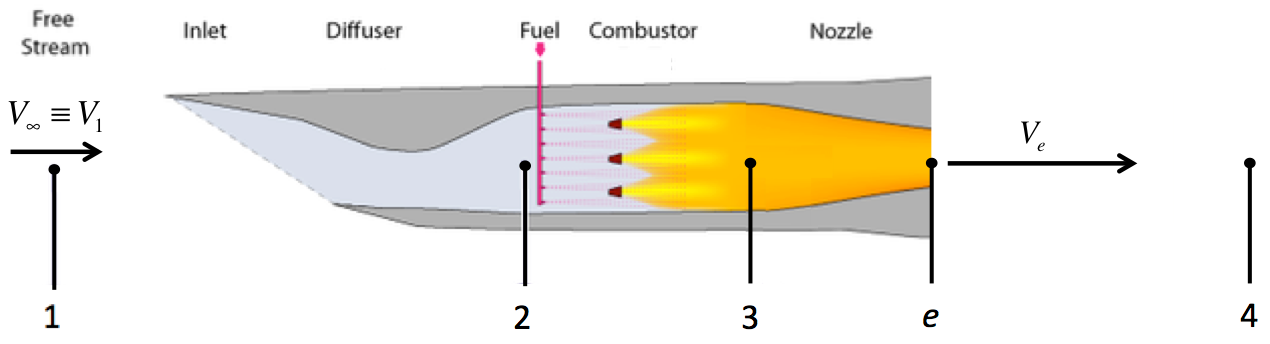
\includegraphics[width=0.75\textwidth]{media/the_ramjet.png}
\caption{\label{fig:propsys} The Ramjet Propulsion System}
\end{figure}

To analyze the ramjet, the analysis tool was broken down into 5 modules focusing on an individual section of the flow path through the jet in Fig. \ref{fig:propsys} and one module for calculating performance parameters.

\begin{table}[hbt!]
\caption{\label{tab:table1} Parametric Analysis Tool Inputs}
\centering
\begin{tabular}{lcc}
\hline
Name& Variable& Units\\\hline
Flight Altitude& $z$& m\\
Flight Mach Number& $M_1$\\
Inlet/Diffuser Efficiency& $\eta_d$\\
Diffuser Exit Mach Number& $M_2$\\
Combustor Exit Max Allowable Total Temperature& $(T_{t3})_{max}$& K\\
Chosen Fuel Heating Value& $q_f$& MJ/kg\\
Nozzle Efficiency& $\eta_n$\\
Nozzle Exit Area& $A_e$& $m^2$\\
\hline
\end{tabular}
\end{table}


\section{Theory}
The

\section{Procedures}
The

\subsection{State 1: Free Stream}
The

\subsection{State 2: Inlet/Diffuser}
The

\subsection{State 3: Combustor}
The

\subsection{State 4: Internal Converging Nozzle Flow}
The

\subsection{State 5: External Flow Past Nozzle Exit}
The

\subsection{Ram/Scramjet Performance Parameters}
The


\section{Results}
The

\subsection{Part A: \textit{T-s} Diagrams for Validation Cases}
The

\begin{figure}[hbt!]
    \centering
    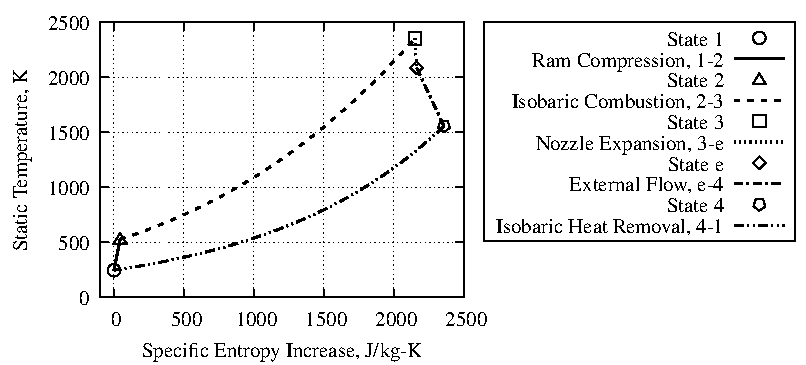
\includegraphics[]{media/ts_plot_files/TS_plot_for_case_7.pdf}
    \caption{\label{fig:partavalida}Validation Case A}
\end{figure}
The

\begin{figure}[hbt!]
    \centering
    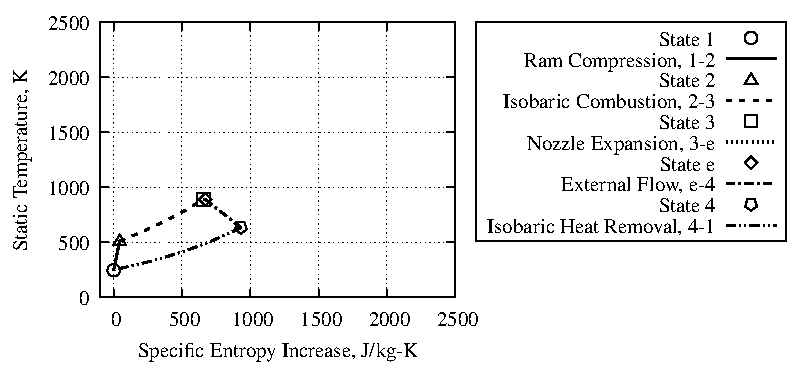
\includegraphics[]{media/ts_plot_files/TS_plot_for_case_8.pdf}
    \caption{\label{fig:partavalidb}Validation Case B}
\end{figure}
The

\subsection{Part B: Atmospheric Model Validation}
The

\begin{figure}[hbt!]
    \centering
    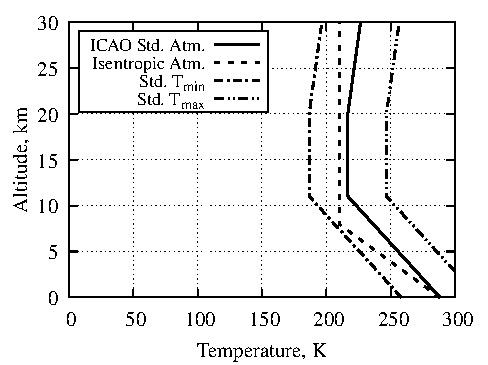
\includegraphics[]{media/atmosphere_validation_files/ICAO_vs_ISEN_temperature.pdf}
    \caption{\label{fig:partbtemp}ICAO Standard Atmosphere vs Isentropic Model (Temperature)}
\end{figure}
The

\begin{figure}[hbt!]
    \centering
    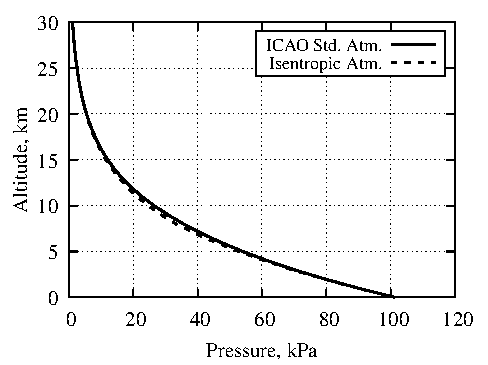
\includegraphics[]{media/atmosphere_validation_files/ICAO_vs_ISEN_pressure.pdf}
    \caption{\label{fig:partbpres}ICAO Standard Atmosphere vs Isentropic Model (Pressure)}
\end{figure}
The

\subsection{Part C: Effect of Flight Mach Number}
The

\subsubsection{Overall Efficiency}
The

\begin{figure}[hbt!]
    \centering
    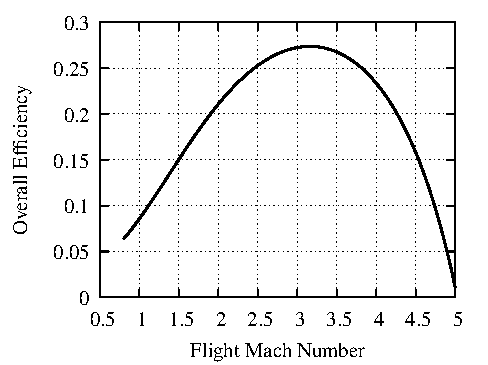
\includegraphics[]{media/performance_parameter_files/part_c_eta_o.pdf}
    \caption{\label{fig:partcetao}Overall Efficiency vs Flight Mach Number}
\end{figure}
The

\subsubsection{Total Thrust}
The

\begin{figure}[hbt!]
    \centering
    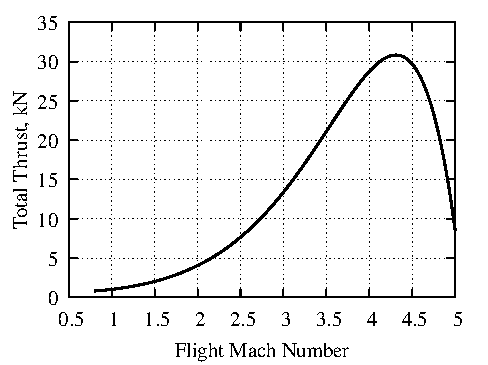
\includegraphics[]{media/performance_parameter_files/part_c_T.pdf}
    \caption{\label{fig:partct}Total Thrust vs Flight Mach Number}
\end{figure}
The

\subsubsection{Thrust Specific Fuel Consumption}
The

\begin{figure}[hbt!]
    \centering
    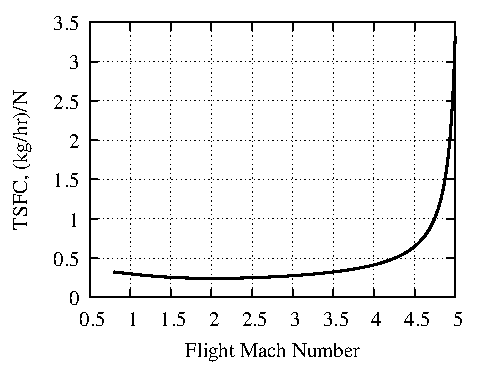
\includegraphics[]{media/performance_parameter_files/part_c_TSFC.pdf}
    \caption{\label{fig:partctsfc}TSFC vs Flight Mach Number}
\end{figure}
The

\subsection{Part D: Effect of Flight Altitude}
The

\subsubsection{Overall Efficiency}
The

\begin{figure}[hbt!]
    \centering
    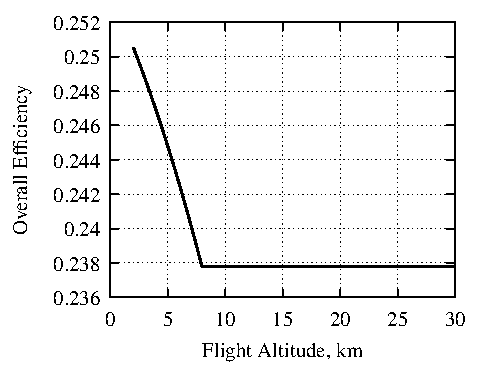
\includegraphics[]{media/performance_parameter_files/part_d_eta_o.pdf}
    \caption{\label{fig:partdetao}Overall Efficiency vs Flight Altitude}
\end{figure}
The

\subsubsection{Total Thrust}
The

\begin{figure}[hbt!]
    \centering
    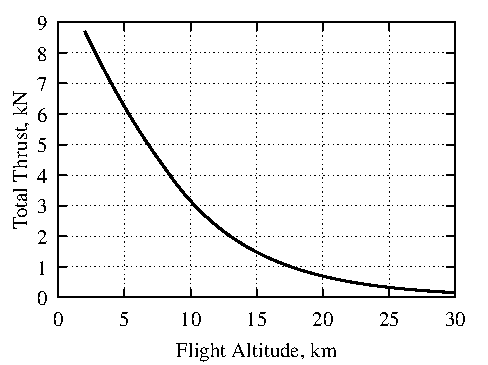
\includegraphics[]{media/performance_parameter_files/part_d_T.pdf}
    \caption{\label{fig:partdt}Total Thrust vs Flight Altitude}
\end{figure}
The

\subsubsection{Thrust Specific Fuel Consumption}
The

\begin{figure}[hbt!]
    \centering
    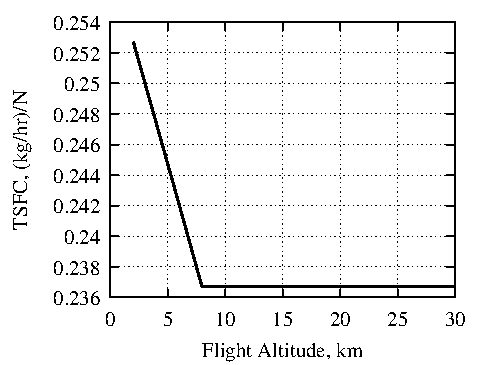
\includegraphics[]{media/performance_parameter_files/part_d_TSFC.pdf}
    \caption{\label{fig:partdtsfc}TSFC vs Flight Altitude}
\end{figure}
The

\subsection{Part E: Optimizing TSFC}
The

\begin{figure}[hbt!]
    \centering
    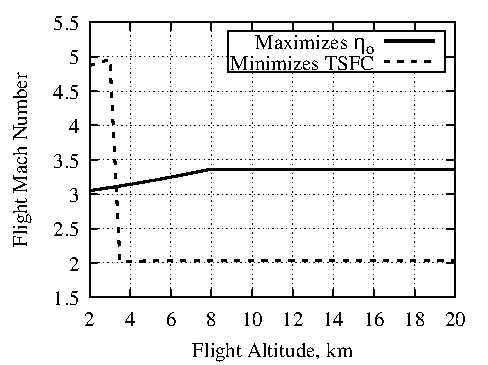
\includegraphics[]{media/performance_parameter_files/part_e_range_1_5.pdf}
    \caption{\label{fig:parte1-5}Optimizing Overall Efficiency and TSFC, Mach 1-5}
\end{figure}

\begin{figure}[hbt!]
    \centering
    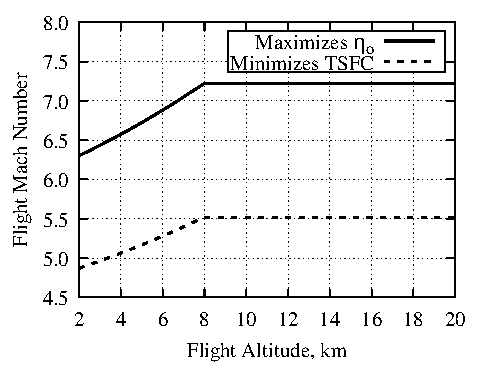
\includegraphics[]{media/performance_parameter_files/part_e_range_1_10.pdf}
    \caption{\label{fig:parte1-10}Optimizing Overall Efficiency and TSFC, Mach 1-10}
\end{figure}

\subsection{Part F: Effect of Inlet/Diffuser Efficiency}
The

\subsubsection{Overall Efficiency}
The

\begin{figure}[hbt!]
    \centering
    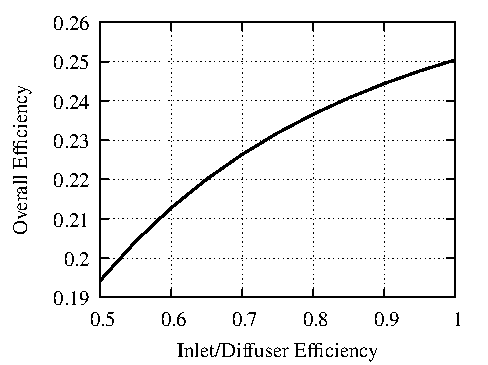
\includegraphics[]{media/performance_parameter_files/part_f_eta_o.pdf}
    \caption{\label{fig:partfetao}Overall Efficiency vs Inlet/Diffuser Efficiency}
\end{figure}
The

\subsubsection{Total Thrust}
The

\begin{figure}[hbt!]
    \centering
    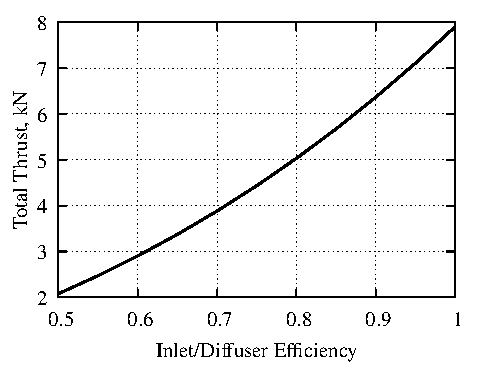
\includegraphics[]{media/performance_parameter_files/part_f_T.pdf}
    \caption{\label{fig:partft}Total Thrust vs Inlet/Diffuser Efficiency}
\end{figure}
The

\subsubsection{Thrust Specific Fuel Consumption}
The

\begin{figure}[hbt!]
    \centering
    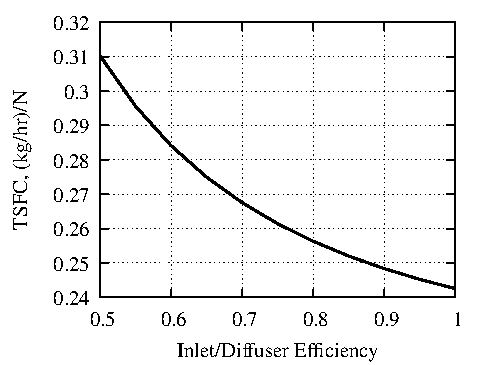
\includegraphics[]{media/performance_parameter_files/part_f_TSFC.pdf}
    \caption{\label{fig:partftsfc}TSFC vs Inlet/Diffuser Efficiency}
\end{figure}
The

\subsection{Part G: Effect of Nozzle Efficiency}
The

\subsubsection{Overall Efficiency}
The

\begin{figure}[hbt!]
    \centering
    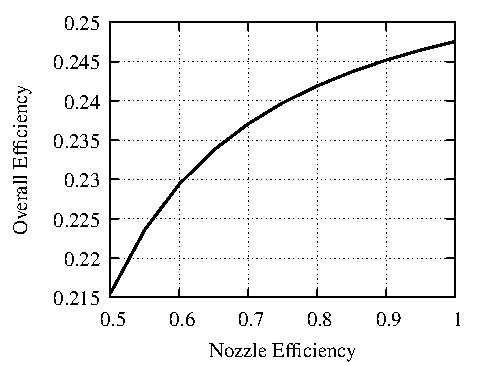
\includegraphics[]{media/performance_parameter_files/part_g_eta_o.pdf}
    \caption{\label{fig:partgetao}Overall Efficiency vs Nozzle Efficiency}
\end{figure}
The

\subsubsection{Total Thrust}
The

\begin{figure}[hbt!]
    \centering
    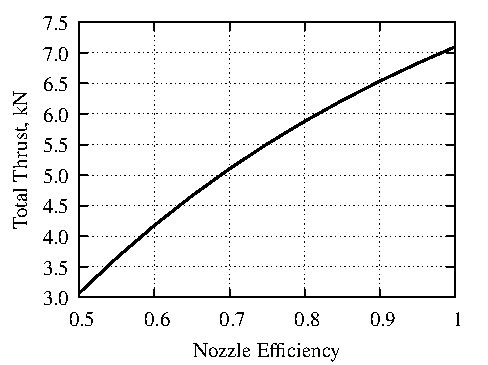
\includegraphics[]{media/performance_parameter_files/part_g_T.pdf}
    \caption{\label{fig:partgt}Total Thrust vs Nozzle Efficiency}
\end{figure}
The

\subsubsection{Thrust Specific Fuel Consumption}
The

\begin{figure}[hbt!]
    \centering
    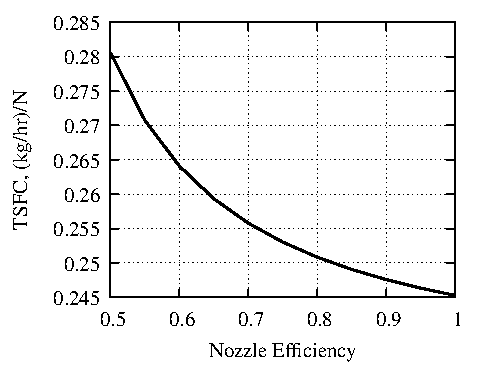
\includegraphics[]{media/performance_parameter_files/part_g_TSFC.pdf}
    \caption{\label{fig:partgtsfc}TSFC vs Nozzle Efficiency}
\end{figure}
The

\subsection{Part H: Effect of \texorpdfstring{\textit{$M_2$}}{M2}}
The

\subsubsection{Overall Efficiency}
The

\begin{figure}[hbt!]
    \centering
    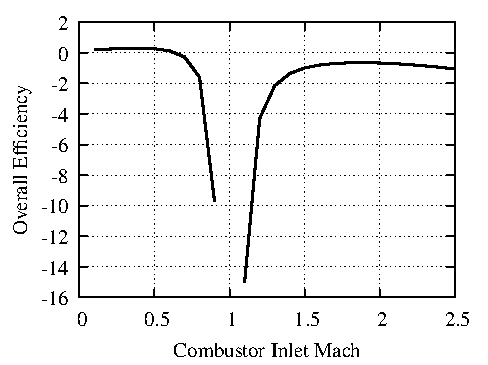
\includegraphics[]{media/performance_parameter_files/part_h_eta_o.pdf}
    \caption{\label{fig:parthetao}Overall Efficiency vs \texorpdfstring{\textit{$M_2$}}{M2}}
\end{figure}
The

\subsubsection{Total Thrust}
The

\begin{figure}[hbt!]
    \centering
    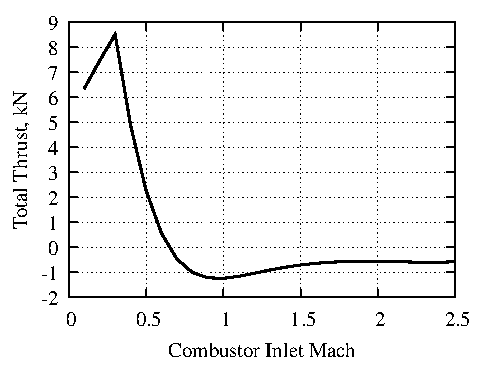
\includegraphics[]{media/performance_parameter_files/part_h_T.pdf}
    \caption{\label{fig:partht}Total Thrust vs \texorpdfstring{\textit{$M_2$}}{M2}}
\end{figure}
The

\subsubsection{Thrust Specific Fuel Consumption}
The

\begin{figure}[hbt!]
    \centering
    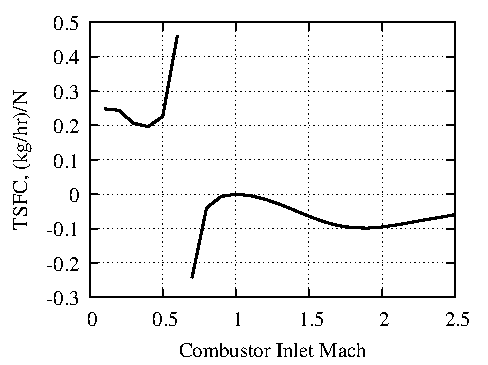
\includegraphics[]{media/performance_parameter_files/part_h_TSFC.pdf}
    \caption{\label{fig:parthtsfc}TSFC vs \texorpdfstring{\textit{$M_2$}}{M2}}
\end{figure}
The

\subsection{Part I: Optimzed Ram/Scramjet Propulsion System}
The

\begin{figure}[hbt!]
    \centering
    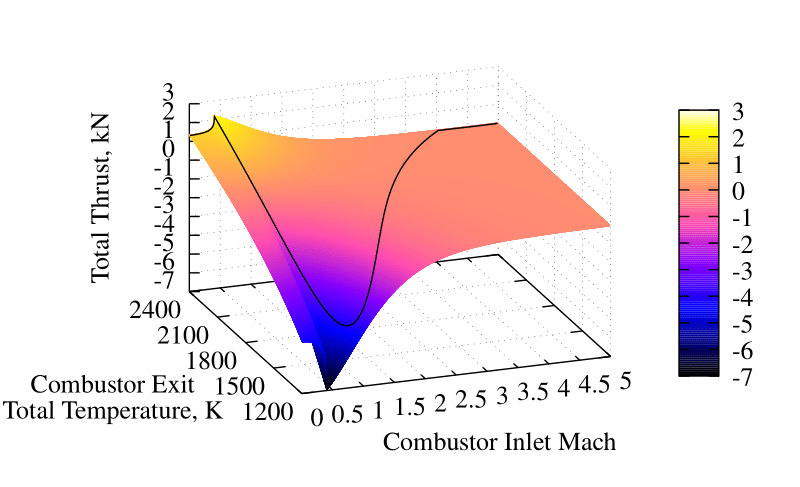
\includegraphics[]{media/propulsion_design_files/total_thrust_plot.pdf}
    \caption{\label{fig:partithrust}Total Thrust}
\end{figure}
The

\begin{figure}[hbt!]
    \centering
    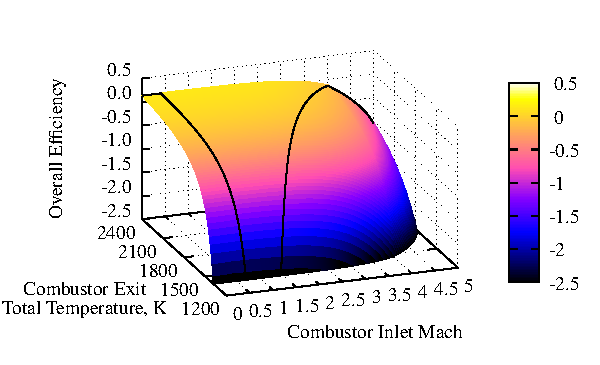
\includegraphics[]{media/propulsion_design_files/eta_o_plot.pdf}
    \caption{\label{fig:partietao}Overall Efficiency}
\end{figure}
The


\section{Conclusion}
Although a conclusion may review the main points of the paper, it must not replicate the abstract. A conclusion might elaborate on the importance of the work or suggest applications and extensions. Do not cite references in the conclusion. Note that the conclusion section is the last section of the paper to be numbered. The appendix (if present), funding information, other acknowledgments, and references are listed without numbers.


\section*{Appendix}
\subsection{Universal Module Code}
\lstinputlisting[language=FORTRAN,basicstyle=\ttfamily\small]{modules/universal_module.f90}

\subsection{Module 1 Code}
\lstinputlisting[language=FORTRAN,basicstyle=\ttfamily\small]{modules/module_1.f90}

\subsection{Module 2 Code}
\lstinputlisting[language=FORTRAN,basicstyle=\ttfamily\small]{modules/module_2.f90}

\subsection{Module 3 Code}
\lstinputlisting[language=FORTRAN,basicstyle=\ttfamily\small]{modules/module_3.f90}

\subsection{Module 4 Code}
\lstinputlisting[language=FORTRAN,basicstyle=\ttfamily\small]{modules/module_4.f90}

\subsection{Module 5 Code}
\lstinputlisting[language=FORTRAN,basicstyle=\ttfamily\small]{modules/module_5.f90}

\subsection{Module 6 Code}
\lstinputlisting[language=FORTRAN,basicstyle=\ttfamily\small]{modules/module_6.f90}

\subsection{Auxiliary Module Code}
\lstinputlisting[language=FORTRAN,basicstyle=\ttfamily\small]{modules/auxiliary_module.f90}


\bibliography{sample}

\end{document}
